\documentclass[../main]{subfiles}

\begin{document}

\section{主翼面積S, エンジン推力$T_{TO}$,揚力係数$C_L$の見積もり}
  \subsection{揚抗比L/D,抵抗Dの推算}
    教科書の例のBWD機を参考にする。
    \begin{equation}
      AR = 9.0
    \end{equation}
    とし,$S_{wet}/S$は,BWD機であるので,
    \begin{equation}
      \frac{S_{wet}}{S} = 3.0
    \end{equation}
    とする.すると配布プリント図4.3の図より,
    \begin{align}
      \frac{AR}{S_{wet}/S} = 3.0 \\[5mm]
      { \biggl( \frac{L}{D} \biggr) }_{max} = 23.0
    \end{align}
    と推算できる.よって,
    \begin{eqnarray}
      \begin{cases}
        { \biggl( \dfrac{L}{D} \biggr) }_{cruise} = 0.866 { \biggl( \dfrac{L}{D} \biggr) }_{max}
        = 20.4 \\[5mm]
        { \biggl( \dfrac{L}{D} \biggr) }_{loiter} = { \biggl( \dfrac{L}{D} \biggr) }_{max}
        = 23.0
     \end{cases}
    \end{eqnarray}
    となり、これは2.1節(7)にて,
    \begin{eqnarray}
      \begin{cases}
        \biggl( \dfrac{L}{D} \biggr) = \biggl( \dfrac{L}{D_{alt}} \biggr)
        = 20 \\[5mm]
        \biggl( \dfrac{L}{D_{loiter}} \biggr) = 23 \\
      \end{cases}
    \end{eqnarray}
    としたことと矛盾しない.また、統計データより,
    \begin{equation}
      C_{f_e} = 0.003
    \end{equation}
    より、
    \begin{equation}
      C_{D_0} = C_{f_e} \frac{S_{wet}}{S} = 0.0090
    \end{equation}
    となり,
    \begin{equation}
      e = 0.80
    \end{equation}
    とすると,クリーン形態では
    \begin{equation}
      C_D = C_{D_0} + \frac{{C_L}^2}{e \pi AR} = 0.0090 + 0.0442 {C_L}^2
    \end{equation}
    またフラップと脚を動作させた状態では,
    \begin{align}
      \text{離陸フラップ:} \quad \Delta C_{D_0} &= 0.015, \quad e=0.75  \\
      \text{着陸フラップ:} \quad \Delta C_{D_0} &= 0.065, \quad e=0.70  \\
      \text{脚出しにより:} \quad \Delta C_{D_0} &= 0.020
    \end{align}
    となるので,
    \begin{align}
      \text{離陸時(脚収納):} \quad C_D &= 0.0240 + 0.0228 {C_L}^2 \\
      \text{離陸時(脚出し):} \quad C_D &= 0.0440 + 0.0228 {C_L}^2 \\
      \text{着陸時(脚収納):} \quad C_D &= 0.0740 + 0.0236 {C_L}^2 \\
      \text{着陸時(脚出し):} \quad C_D &= 0.0940 + 0.0236 {C_L}^2
    \end{align}
    が得られる.

  \subsection{離陸性能のサイジング}
    離陸性能の際のサイジングの代表値として,
    \begin{equation}
      C_{L_{max}TO} = 1.6,2.0,2.4
    \end{equation}
    を用いる.
    統計関係式より,
    \begin{equation}
      S_{TOFL} = 40.3 \times \dfrac{(W/S)_{TO}}{\sigma C_{L_{max}TO} \cdot (T/W)_{TO}} = 10000 \ [ft]
    \end{equation}
    という関係が得られる.これを整理すると,代表値それぞれについて,
    \begin{eqnarray}
      \begin{cases}
        (T/W)_{TO} = 0.00252 (W/S)_{TO} \quad at \ C_{L_{max}TO} = 1.6 \\[3mm]
        (T/W)_{TO} = 0.00201 (W/S)_{TO} \quad at \ C_{L_{max}TO} = 2.0 \\[3mm]
        (T/W)_{TO} = 0.00168 (W/S)_{TO} \quad at \ C_{L_{max}TO} = 2.4 \\[3mm]
      \end{cases}
    \end{eqnarray}
    となる.

  \subsection{着陸性能のサイジング}
    着陸性能のサイジング値の代表値として,
    \begin{equation}
      C_{L_{max}L} = 1.8,2.2,2.6,3.0
    \end{equation}
    を用いる.設計要求より,
    \begin{equation}
      S_{FL} = 0.29{V_A}^2 = 0.29 \times {(1.3V_{SL})}^2 = 7000 [ft]
    \end{equation}
    であるから
    \begin{equation}
      V_{SL} = 120 [kt]
    \end{equation}
    となる.
    \begin{equation}
      {(W/S)}_{TO} = \frac{\frac{1}{2}\rho {V_{SL}}^2 C_{L_{max}L}}{W_L/W_{TO}}
    \end{equation}
    ここで
    \begin{equation}
      W_L/W_{TO} = 0.80, \quad \rho = 1.225[kg/m^3] = 0.125[kg \cdot s^2/m^4]
    \end{equation}
    であるから,代表値それぞれについて,
    \begin{eqnarray}
      \begin{cases}
        (W/S)_{TO} = 108.8 \ [Ib/{ft}^2] \quad at \quad  C_{L_{max}L}=1.8 \\[3mm]
        (W/S)_{TO} = 133.0 \ [Ib/{ft}^2] \quad at \quad  C_{L_{max}L}=2.2 \\[3mm]
        (W/S)_{TO} = 157.2 \ [Ib/{ft}^2] \quad at \quad  C_{L_{max}L}=2.6 \\[3mm]
        (W/S)_{TO} = 181.4 \ [Ib/{ft}^2] \quad at \quad  C_{L_{max}L}=3.0 \\[3mm]
      \end{cases}
    \end{eqnarray}
    となる.

  \subsection{上昇性能のサイジング}
    上昇性能のサイジングは, FAR25の機体において最も厳しい要求である,second segment climb
    requirements(OEI)についてのみ行う.設計機体は3発機であるから,上昇勾配$\gamma$
    について
    \begin{equation}
      \gamma > 0.027
    \end{equation}
    であるので,
    \begin{equation}
      {(T/W)}_{TO} = \frac{3}{2} \biggl( \frac{1}{L/D} + 0.027 \biggr) \quad at \ 1.2V_{STO}
    \end{equation}
    となる.second segment climb requirement においては, 離陸時脚収納状態であるから,
    式(14)より,
    \begin{equation}
      C_D = 0.0240 + 0.0228 {C_L}^2 = 0.087
    \end{equation}
    であるから,
    \begin{equation}
      \frac{L}{D} = \frac{C_L}{C_D} = 19.1
    \end{equation}
    となる.よって式(28)にこれを代入して,
    \begin{equation}
      {(T/W)}_{TO} = 0.119
    \end{equation}
    これに標準待機状態より気温が$27.8[^\circ C]$高い影響で推力が$20\%$ほど低下する影響を
    加味して,
    \begin{equation}
      {(T/W)}_{TO} = \frac{0.119}{0.8} = 0.149
    \end{equation}
    となる.
  \subsection{巡航速度のサイジング}
    巡航時の関係式は
    \begin{equation}
      {\biggl( \frac{T}{W} \biggr) }_{cr} = \frac{(C_{D_0}+ \Delta C_{D_0})q}{W/S} + \frac{W/S}{qe \pi AR}
    \end{equation}
    となる.
    ここで、標準大気表より、高度38000[ft]での巡航時動圧q
    \begin{align}
      q &= \frac{1}{2} \rho V^2 \\
        &= \frac{1}{2} \times 0.272 \times 0.125 [kg \cdot s^2/m^4] \times \
        (M 0.8 \times 0.867 \times 340.3[m/s]) \\
        &= 194[Ib/ft^2]
    \end{align}
    また圧縮性の影響より
    \begin{equation}
      \Delta C_{D_0} = 0.0030
    \end{equation}
    設計要求より,
    \begin{equation}
      L_{p_{cr}} = 0.167
    \end{equation}
    また
    \begin{equation}
      \frac{W_{cr}}{W_{TO}} = \frac{W_1}{W_{TO}}\frac{W_2}{W_1}\frac{W_3}{W_2}\frac{W_4}{W_3}
      = 0.956
    \end{equation}
    よって、これらの値を用いて,
    \begin{equation}
      {(T/W)}_{TO} = \dfrac{({\frac{T}{W})}_{cr} (\frac{W_{cr}}{W_{TO}})}{L_{p_{cr}}}
      = 5.72 \biggl ( \frac{2.43}{{(W/S)}_{TO}} + \frac{{(W/S)}_{TO}}{4585} \biggr)
    \end{equation}
    を得る.
  \subsection{サイジングプロット}
  3.2~3.5節からサイジングプロットを描くと,下図のようになる.
  \begin{figure}[H]
    \begin{center}
      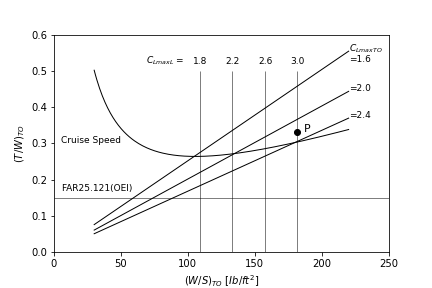
\includegraphics[width=12.0cm]{sizing.png}
      \caption{420人乗りBWB機のサイジング結果} %タイトルをつける
      \label{sizing} %ラベルをつけ図の参照を可能にする
    \end{center}
  \end{figure}
  ここでは,上図のP点($C_{L_{max}L} = 3.0 , C_{L_{max}TO} = 2.2$)を設計点とする.
  すると,
  \begin{eqnarray}
    \begin{cases}
      {(T/W)}_{TO} = 0.3323 \\
      {(W/S)}_{TO} = 181 \ [Ib/ft^2] \\
    \end{cases}
  \end{eqnarray}
  となるので,先に得られた$W_{TO} = 896000 [Ibs]$より,
  \begin{eqnarray}
    \begin{cases}
      T = 297756 \ [Ib]\\
      S = 4938.9 \ [ft^2] \\
    \end{cases}
  \end{eqnarray}
  を得る.
\end{document}
